% !TEX TS-program = pdflatex
\documentclass[11pt]{article}

% -------------------- Packages --------------------
\usepackage[a4paper,margin=1in]{geometry}
\usepackage{amsmath,amssymb}
\usepackage[T1]{fontenc}
\usepackage{lmodern}
\usepackage{xcolor}
\usepackage{tcolorbox}
\tcbuselibrary{skins,breakable}
\usepackage{enumitem}
\usepackage{hyperref}
\usepackage{tikz}
\usetikzlibrary{arrows.meta,calc}

\pagestyle{empty}

% -------------------- Dark Theme Colors --------------------
\definecolor{bg}{HTML}{000000}
\definecolor{pairbg}{HTML}{121212}
\definecolor{solbg}{HTML}{0A0A0A}
\definecolor{border}{HTML}{2A2A2A}
\definecolor{text}{HTML}{FFFFFF}
\definecolor{muted}{HTML}{C9CDD3}
\definecolor{gold}{HTML}{FFD700}
\definecolor{green}{HTML}{4ADE80}
\definecolor{cyan}{HTML}{38BDF8}

\pagecolor{bg}
\color{text}

\hypersetup{
  colorlinks=true,
  linkcolor=cyan,
  urlcolor=cyan
}

\setlength{\parindent}{0pt}
\setlength{\parskip}{10pt}

% Prevent right-overflow in tight boxes
\setlength{\emergencystretch}{2em}

\setlist[itemize]{left=1.4em,itemsep=6pt,topsep=6pt}
\setlist[enumerate]{left=1.6em,itemsep=4pt,topsep=4pt}

% -------------------- tcolorbox Base --------------------
\tcbset{
  enhanced,
  breakable,
  arc=12pt,
  boxrule=0.8pt,
  left=16pt,right=16pt,top=12pt,bottom=12pt
}

\newtcolorbox{QAPair}[1]{%
  colback=pairbg,
  colbacklower=solbg,
  colframe=border,
  coltext=text,
  title=\textcolor{gold}{\bfseries #1},
  fonttitle=\bfseries,
  coltitle=text,
  segmentation style={draw=border, dashed, line width=0.6pt},
  before upper=\raggedright,
  before lower=\raggedright,
}

\newtcolorbox{QuickBox}{%
  colback=pairbg,
  colframe=cyan,
  coltext=text,
  fontupper=\color{text}\raggedright,
  borderline north={4pt}{0pt}{cyan},
  arc=14pt,
  boxrule=0.8pt
}

% Helper for step headings
\newcommand{\Step}[1]{\textcolor{muted}{\textbf{Step #1:}}}

% -------------------- TikZ helpers (fast diagrams) --------------------
\tikzset{
  ax/.style={-Stealth, thick, draw=text},
  gridline/.style={very thin, draw=border},
  vcyan/.style={-Stealth, very thick, draw=cyan},
  vgreen/.style={-Stealth, very thick, draw=green},
  vgold/.style={-Stealth, very thick, draw=gold},
  vmuted/.style={-Stealth, thick, draw=muted},
  pt/.style={circle, fill=gold, draw=gold, inner sep=1.6pt}
}

\newcommand{\DrawAxes}[4]{% xmin,xmax,ymin,ymax
  \draw[ax] (#1,0) -- (#2,0) node[right]{\textcolor{muted}{$x$ (East)}};
  \draw[ax] (0,#3) -- (0,#4) node[above]{\textcolor{muted}{$y$ (North)}};
}

\newcommand{\TinyNote}[1]{\textcolor{muted}{\footnotesize #1}}

% ============================================================
\begin{document}

\begin{center}
{\LARGE\bfseries \textcolor{gold}{Exercise 7.1 --- Solutions}}\\[-2pt]
\end{center}

\begin{QuickBox}
{\color{cyan}\bfseries Quick formulas (Vectors)}\par\medskip
\begin{itemize}
\item \textbf{Component form:} $\vec v=\langle x,y\rangle = x\hat{\imath}+y\hat{\jmath}$.
\item \textbf{Magnitude:} $|\vec v|=\sqrt{x^2+y^2}$.
\item \textbf{Unit vector:} $\hat v=\dfrac{\vec v}{|\vec v|}$ (same direction, length $1$).
\item \textbf{Angle with +x-axis:} if $|\vec v|=r$ and angle is $\theta$, then
$\vec v=\langle r\cos\theta,\, r\sin\theta\rangle$.
\item \textbf{Translation:} $(x,y)$ translated by $\langle a,b\rangle$ becomes $(x+a,\;y+b)$.
\item \textbf{Bearings (measured clockwise from North):} for speed $s$ and bearing $\theta$,
\[
\text{East} = s\sin\theta,\qquad \text{North} = s\cos\theta.
\]
\end{itemize}
\end{QuickBox}

% ============================================================
% Q1
\begin{QAPair}{Question 1}
\textcolor{gold}{\bfseries Question:} Draw the following vectors:
(i) $10$ N force along $x$-axis,\;
(ii) $50$ m/s at $150^\circ$ with $x$-axis,\;
(iii) $220$ m towards north,\;
(iv) $24$ m/s$^2$ at $45^\circ$ with $x$-axis.
\tcblower
\textcolor{green}{\bfseries Answer:}

(Take $+x$ to the right and $+y$ upward/north.)

\[
\begin{aligned}
\text{(i)}\;& \vec F=\langle 10,0\rangle = 10\hat{\imath}.\\[4pt]
\text{(ii)}\;& \vec v=\langle 50\cos150^\circ,\;50\sin150^\circ\rangle
=\left\langle -25\sqrt3,\;25\right\rangle
= -25\sqrt3\,\hat{\imath}+25\,\hat{\jmath}.\\[4pt]
\text{(iii)}\;& \vec s=\langle 0,220\rangle = 220\,\hat{\jmath}.\\[4pt]
\text{(iv)}\;& \vec a=\langle 24\cos45^\circ,\;24\sin45^\circ\rangle
=\langle 12\sqrt2,\;12\sqrt2\rangle
=12\sqrt2\,\hat{\imath}+12\sqrt2\,\hat{\jmath}.
\end{aligned}
\]

\begin{center}
\begin{tikzpicture}[scale=0.75]
  \DrawAxes{-6}{6}{-1}{6}
  % Not-to-scale drawing (direction matters)
  \draw[vcyan]  (0,0) -- (4,0) node[below right]{\textcolor{cyan}{(i)}};
  \draw[vgreen] (0,0) -- (-4.33,2.5) node[above left]{\textcolor{green}{(ii)}};
  \draw[vgold]  (0,0) -- (0,5) node[above right]{\textcolor{gold}{(iii)}};
  \draw[vmuted] (0,0) -- (3.4,3.4) node[above right]{\textcolor{muted}{(iv)}};
\end{tikzpicture}

\TinyNote{Diagram is scaled for drawing; directions are the key.}
\end{center}
\end{QAPair}

% ============================================================
% Q2
\begin{QAPair}{Question 2}
\textcolor{gold}{\bfseries Question:} On graph paper, $\vec p$ is $4$ cm long making $45^\circ$ with $x$-axis. Draw:
(i) $2\vec p$ \; (ii) $-\vec p$ \; (iii) $0.5\vec p$ \; (iv) $1.5\vec p$ \; (v) $-0.5\vec p$.
\tcblower
\textcolor{green}{\bfseries Answer:}

\Step{1} $\vec p$ has length $4$ cm and angle $45^\circ$ (NE direction).\par
\Step{2} Scalar multiples change the length by $|k|$ and keep/reverse the direction:\par

\begin{itemize}
\item (i) $2\vec p$: same direction as $\vec p$, length $2\times 4=8$ cm.
\item (ii) $-\vec p$: opposite direction, length $4$ cm.
\item (iii) $0.5\vec p$: same direction, length $0.5\times 4=2$ cm.
\item (iv) $1.5\vec p$: same direction, length $1.5\times 4=6$ cm.
\item (v) $-0.5\vec p$: opposite direction, length $0.5\times 4=2$ cm.
\end{itemize}

\begin{center}
\begin{tikzpicture}[scale=0.8]
  \DrawAxes{-6}{6}{-6}{6}
  % Use simple approximations for 45 degrees
  \draw[vcyan]  (0,0) -- (2.8,2.8) node[above right]{\textcolor{cyan}{$\vec p$}};
  \draw[vgreen] (0,0) -- (5.6,5.6) node[above right]{\textcolor{green}{$2\vec p$}};
  \draw[vmuted] (0,0) -- (4.2,4.2) node[above right]{\textcolor{muted}{$1.5\vec p$}};
  \draw[vgold]  (0,0) -- (1.4,1.4) node[above right]{\textcolor{gold}{$0.5\vec p$}};
  \draw[vcyan,dashed] (0,0) -- (-2.8,-2.8) node[below left]{\textcolor{cyan}{$-\vec p$}};
  \draw[vgreen,dashed] (0,0) -- (-1.4,-1.4) node[below left]{\textcolor{green}{$-0.5\vec p$}};
\end{tikzpicture}

\TinyNote{Opposite direction is shown with dashed arrows.}
\end{center}
\end{QAPair}

% ============================================================
% Q3
\begin{QAPair}{Question 3}
\textcolor{gold}{\bfseries Question:} $\vec a=3$ units west and $\vec b=3$ units north. Draw:
(i) $2\vec a+\vec b$ (ii) $\vec a-2\vec b$ (iii) $3\vec a+1.5\vec b$
(iv) $(2\vec a+\vec b)+(\vec a-2\vec b)$ (v) $0.5(\vec a+\vec b)$
(vi) $3\vec a-2\vec b$ (vii) $2\vec a-2.5\vec b$ (viii) $(2\vec a+\vec b)-(\vec a-2\vec b)$.
\tcblower
\textcolor{green}{\bfseries Answer:}

\Step{1} $\vec a=\langle -3,0\rangle,\qquad \vec b=\langle 0,3\rangle.$

\[
\begin{aligned}
\text{(i)}\;& 2\vec a+\vec b = \langle-6,3\rangle.\\
\text{(ii)}\;& \vec a-2\vec b=\langle-3,-6\rangle.\\
\text{(iii)}\;& 3\vec a+1.5\vec b=\left\langle-9,\tfrac{9}{2}\right\rangle.\\
\text{(iv)}\;& (2\vec a+\vec b)+(\vec a-2\vec b)=\langle-9,-3\rangle.\\
\text{(v)}\;& 0.5(\vec a+\vec b)=\left\langle -\tfrac{3}{2},\tfrac{3}{2}\right\rangle.\\
\text{(vi)}\;& 3\vec a-2\vec b=\langle-9,-6\rangle.\\
\text{(vii)}\;& 2\vec a-2.5\vec b=\left\langle-6,-\tfrac{15}{2}\right\rangle.\\
\text{(viii)}\;& (2\vec a+\vec b)-(\vec a-2\vec b)=\langle-3,9\rangle.
\end{aligned}
\]

\begin{center}
\begin{tikzpicture}[scale=0.75]
  \DrawAxes{-10}{4}{-8}{10}
  \draw[vmuted] (0,0) -- (-3,0) node[below left]{\textcolor{muted}{$\vec a$}};
  \draw[vmuted] (0,0) -- (0,3) node[above right]{\textcolor{muted}{$\vec b$}};

  % Example resultants for drawing practice
  \draw[vcyan]  (0,0) -- (-6,3) node[above left]{\textcolor{cyan}{$2\vec a+\vec b$}};
  \draw[vgreen] (0,0) -- (-3,-6) node[below left]{\textcolor{green}{$\vec a-2\vec b$}};
\end{tikzpicture}

\TinyNote{Use the component answers to plot each requested vector.}
\end{center}
\end{QAPair}

% ============================================================
% Q4
\begin{QAPair}{Question 4}
\textcolor{gold}{\bfseries Question:} In the figure, $\vec a$ is $4$ squares right and $3$ squares up. Find the relation of other vectors with $\vec a$.
\tcblower
\textcolor{green}{\bfseries Answer:}

\Step{1} $\vec a=\langle 4,3\rangle$ (in square units).\par
\Step{2} Each shown vector is parallel to $\vec a$, so it is a scalar multiple of $\vec a$.\par

By counting squares (same direction = positive multiple, opposite direction = negative multiple):
\[
\boxed{
\begin{aligned}
\vec b&=-\tfrac12\vec a,\quad \vec c=2\vec a,\quad \vec d=-\vec a,\\
\vec e&=3\vec a,\quad \vec f=\tfrac12\vec a,\quad \vec g=-2\vec a.
\end{aligned}}
\]

\begin{center}
\begin{tikzpicture}[scale=0.7]
  \DrawAxes{-10}{10}{-10}{10}
  \draw[vcyan] (0,0) -- (4,3) node[above right]{\textcolor{cyan}{$\vec a$}};
  \draw[vgreen] (0,0) -- (8,6) node[above right]{\textcolor{green}{$2\vec a$}};
  \draw[vmuted] (0,0) -- (2,1.5) node[above right]{\textcolor{muted}{$\tfrac12\vec a$}};
  \draw[vgold,dashed] (0,0) -- (-4,-3) node[below left]{\textcolor{gold}{$-\vec a$}};
\end{tikzpicture}
\end{center}
\end{QAPair}

% ============================================================
% Q5
\begin{QAPair}{Question 5}
\textcolor{gold}{\bfseries Question:} A point $(5,-7)$ is translated by the vector $\langle 0,-3\rangle$. Find the new position.
\tcblower
\textcolor{green}{\bfseries Answer:}
\[
\begin{aligned}
\Step{1}\;& (x,y)\mapsto(x+0,\;y-3).\\
\Step{2}\;& (5,-7)\mapsto (5,\,-10).
\end{aligned}
\]
\[
\boxed{(5,-10)}
\]

\begin{center}
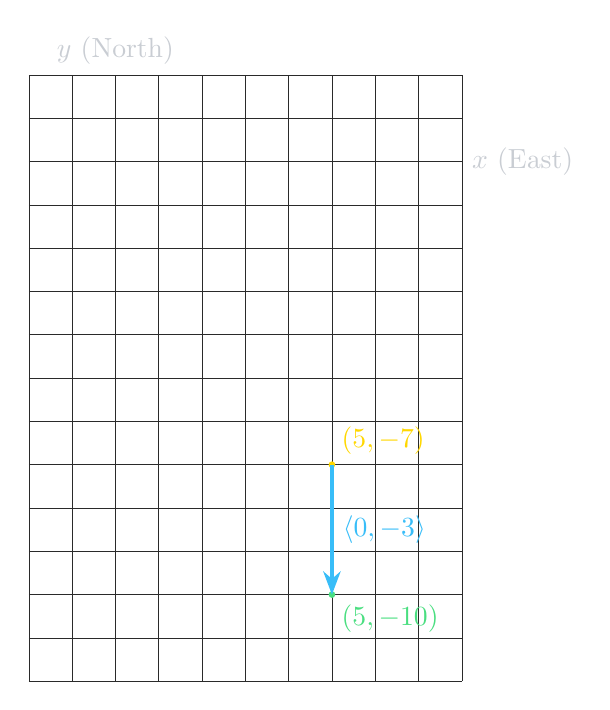
\begin{tikzpicture}[scale=0.55]
  \DrawAxes{-2}{8}{-12}{2}
  \draw[gridline] (-2,-12) grid (8,2);
  \fill[gold] (5,-7) circle (2.2pt) node[above right]{\textcolor{gold}{$(5,-7)$}};
  \fill[green] (5,-10) circle (2.2pt) node[below right]{\textcolor{green}{$(5,-10)$}};
  \draw[vcyan] (5,-7) -- (5,-10) node[midway,right]{\textcolor{cyan}{$\langle 0,-3\rangle$}};
\end{tikzpicture}
\end{center}
\end{QAPair}

% ============================================================
% Q6
\begin{QAPair}{Question 6}
\textcolor{gold}{\bfseries Question:} A vector $\langle -5,4\rangle$ is translated by another vector $\langle 4,-3\rangle$. Find the new location of the given vector.
\tcblower
\textcolor{green}{\bfseries Answer:}
\[
\begin{aligned}
\Step{1}\;& \langle -5,4\rangle + \langle 4,-3\rangle
= \langle -5+4,\;4-3\rangle\\
\Step{2}\;&= \langle -1,1\rangle.
\end{aligned}
\]
\[
\boxed{\langle -1,1\rangle}
\]

\begin{center}
\begin{tikzpicture}[scale=0.7]
  \DrawAxes{-7}{5}{-5}{6}
  \draw[vcyan]  (0,0) -- (-5,4) node[above left]{\textcolor{cyan}{$\langle-5,4\rangle$}};
  \draw[vgreen] (-5,4) -- (-1,1) node[above right]{\textcolor{green}{$\langle4,-3\rangle$}};
  \draw[vgold]  (0,0) -- (-1,1) node[above right]{\textcolor{gold}{$\langle-1,1\rangle$}};
  \fill[gold] (-1,1) circle (2.2pt);
\end{tikzpicture}

\TinyNote{Head-to-tail addition: the resultant goes from the start to the final point.}
\end{center}
\end{QAPair}

% ============================================================
% Q7
\begin{QAPair}{Question 7}
\textcolor{gold}{\bfseries Question:} Triangle $ABC$ has vertices
$A(-4,6),\;B(-1,4),\;C(-6,1)$. Find image coordinates if:
(i) translated by $\langle 5,0\rangle$ \quad (ii) translated by $\langle -3,-4\rangle$.
\tcblower
\textcolor{green}{\bfseries Answer:}

\textbf{(i) Translation by $\langle 5,0\rangle$:}
\[
\begin{aligned}
A'&=(-4+5,\;6+0)=(1,6),\\
B'&=(-1+5,\;4+0)=(4,4),\\
C'&=(-6+5,\;1+0)=(-1,1).
\end{aligned}
\]

\textbf{(ii) Translation by $\langle -3,-4\rangle$:}
\[
\begin{aligned}
A''&=(-4-3,\;6-4)=(-7,2),\\
B''&=(-1-3,\;4-4)=(-4,0),\\
C''&=(-6-3,\;1-4)=(-9,-3).
\end{aligned}
\]

\begin{center}
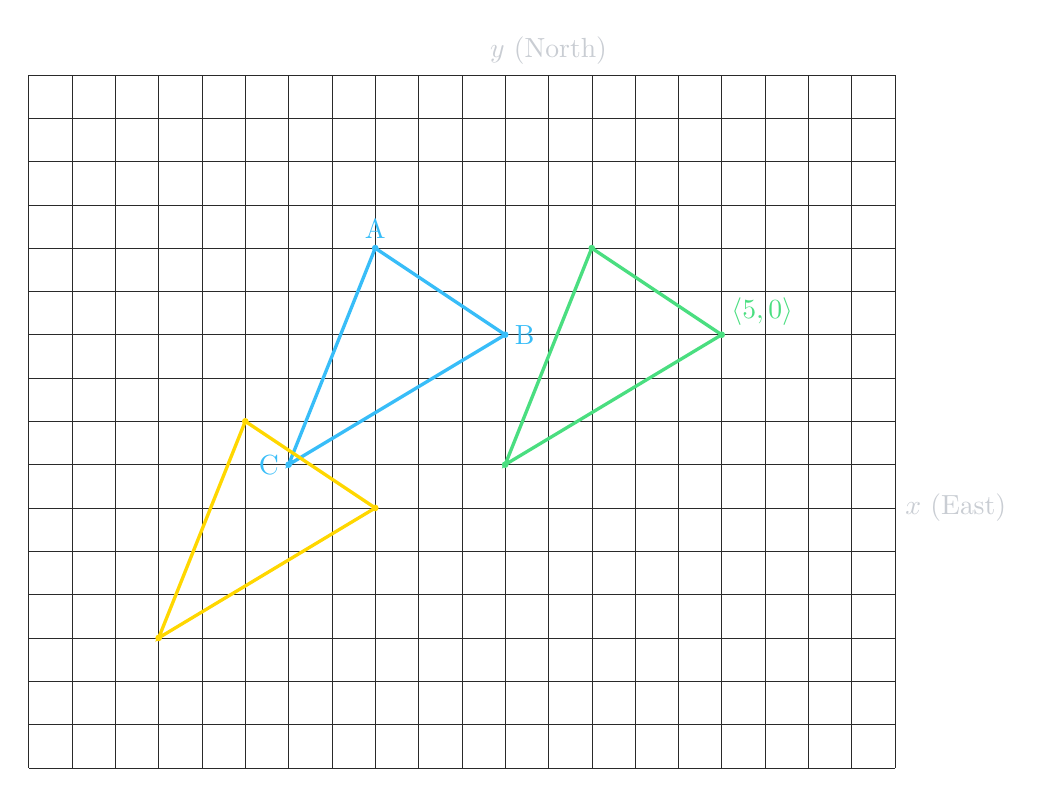
\begin{tikzpicture}[scale=0.55]
  \DrawAxes{-12}{8}{-6}{10}
  \draw[gridline] (-12,-6) grid (8,10);

  % Original triangle
  \coordinate (A) at (-4,6);
  \coordinate (B) at (-1,4);
  \coordinate (C) at (-6,1);
  \draw[vcyan] (A) -- (B) -- (C) -- cycle;
  \fill[cyan] (A) circle (2.2pt) node[above]{\textcolor{cyan}{A}};
  \fill[cyan] (B) circle (2.2pt) node[right]{\textcolor{cyan}{B}};
  \fill[cyan] (C) circle (2.2pt) node[left]{\textcolor{cyan}{C}};

  % Translation (i): +<5,0>
  \coordinate (Ap) at (1,6);
  \coordinate (Bp) at (4,4);
  \coordinate (Cp) at (-1,1);
  \draw[vgreen] (Ap) -- (Bp) -- (Cp) -- cycle;
  \fill[green] (Ap) circle (2.2pt);
  \fill[green] (Bp) circle (2.2pt);
  \fill[green] (Cp) circle (2.2pt);
  \node[above right] at (Bp) {\textcolor{green}{$\langle 5,0\rangle$}};

  % Translation (ii): +<-3,-4>
  \coordinate (Add) at (-7,2);
  \coordinate (Bdd) at (-4,0);
  \coordinate (Cdd) at (-9,-3);
  \draw[vgold] (Add) -- (Bdd) -- (Cdd) -- cycle;
  \fill[gold] (Add) circle (2.2pt);
  \fill[gold] (Bdd) circle (2.2pt);
  \fill[gold] (Cdd) circle (2.2pt);
\end{tikzpicture}

\TinyNote{Cyan = original, Green = after $\langle5,0\rangle$, Gold = after $\langle-3,-4\rangle$.}
\end{center}
\end{QAPair}

% ============================================================
% Q8
\begin{QAPair}{Question 8}
\textcolor{gold}{\bfseries Question:} What translation vector is needed to bring $E(-6,5)$ to the origin?
\tcblower
\textcolor{green}{\bfseries Answer:}
\[
\Step{1}\; \langle a,b\rangle \text{ must satisfy } (-6+a,\;5+b)=(0,0).
\]
\[
\Step{2}\; a=6,\; b=-5.
\]
\[
\boxed{\langle 6,-5\rangle}
\]

\begin{center}
\begin{tikzpicture}[scale=0.7]
  \DrawAxes{-8}{6}{-2}{8}
  \fill[gold] (-6,5) circle (2.2pt) node[above left]{\textcolor{gold}{$E(-6,5)$}};
  \fill[green] (0,0) circle (2.2pt) node[below right]{\textcolor{green}{$O(0,0)$}};
  \draw[vcyan] (-6,5) -- (0,0) node[midway,above]{\textcolor{cyan}{$\langle 6,-5\rangle$}};
\end{tikzpicture}
\end{center}
\end{QAPair}

% ============================================================
% Q9
\begin{QAPair}{Question 9}
\textcolor{gold}{\bfseries Question:} $ABCD$ is a rectangle. Express the following in terms of $\vec a$ and $\vec b$:
(i) $\overrightarrow{DC}$ (ii) $\overrightarrow{DA}$ (iii) $\overrightarrow{AC}$
(iv) $\overrightarrow{BD}$ (v) $\overrightarrow{AO}$ (vi) $\overrightarrow{BO}$ (vii) $\overrightarrow{AB}+\overrightarrow{AC}$.
\tcblower
\textcolor{green}{\bfseries Answer:}

From the figure: $\overrightarrow{AB}=\vec a$ and $\overrightarrow{BC}=\vec b$.

\[
\begin{aligned}
\text{(i)}\;& \overrightarrow{DC}=\vec a.\\
\text{(ii)}\;& \overrightarrow{DA}=-\vec b.\\
\text{(iii)}\;& \overrightarrow{AC}=\vec a+\vec b.\\
\text{(iv)}\;& \overrightarrow{BD}=\vec b-\vec a.\\
\text{(v)}\;& O \text{ midpoint of }AC \Rightarrow \overrightarrow{AO}=\tfrac12(\vec a+\vec b).\\
\text{(vi)}\;& O \text{ midpoint of }BD \Rightarrow \overrightarrow{BO}=\tfrac12(\vec b-\vec a).\\
\text{(vii)}\;& \overrightarrow{AB}+\overrightarrow{AC}=2\vec a+\vec b.
\end{aligned}
\]

\begin{center}
\begin{tikzpicture}[scale=0.9]
  % A simple illustrative rectangle (direction only)
  \coordinate (A) at (0,0);
  \coordinate (B) at (5,0);
  \coordinate (C) at (5,3);
  \coordinate (D) at (0,3);
  \coordinate (O) at (2.5,1.5);

  \draw[gridline] (-0.5,-0.5) grid (5.5,3.5);
  \draw[vmuted] (A) -- (B) -- (C) -- (D) -- cycle;

  \draw[vcyan] (A) -- (B) node[midway,below]{\textcolor{cyan}{$\vec a$}};
  \draw[vgreen] (B) -- (C) node[midway,right]{\textcolor{green}{$\vec b$}};

  \draw[muted,thick,dashed] (A) -- (C);
  \draw[muted,thick,dashed] (B) -- (D);
  \fill[gold] (O) circle (2.2pt) node[above right]{\textcolor{gold}{$O$}};

  \fill[text] (A) circle (2pt) node[below left]{\textcolor{text}{A}};
  \fill[text] (B) circle (2pt) node[below right]{\textcolor{text}{B}};
  \fill[text] (C) circle (2pt) node[above right]{\textcolor{text}{C}};
  \fill[text] (D) circle (2pt) node[above left]{\textcolor{text}{D}};
\end{tikzpicture}

\TinyNote{Diagram is illustrative: any rectangle with adjacent sides $\vec a$ and $\vec b$ gives the same relations.}
\end{center}
\end{QAPair}

% ============================================================
% Q10
\begin{QAPair}{Question 10}
\textcolor{gold}{\bfseries Question:} Given $\overrightarrow{OP}=\vec p+\vec q$, $\overrightarrow{OQ}=\vec p-\vec q$ and $M$ is midpoint of $PQ$. Find:
(i) $\overrightarrow{PQ}$ (ii) $\overrightarrow{PM}$ (iii) $\overrightarrow{QM}$ (iv) $\overrightarrow{OM}$.
\tcblower
\textcolor{green}{\bfseries Answer:}
\[
\begin{aligned}
\text{(i)}\;& \overrightarrow{PQ}=\overrightarrow{OQ}-\overrightarrow{OP}
=(\vec p-\vec q)-(\vec p+\vec q)=-2\vec q.\\
\text{(ii)}\;& M \text{ midpoint of }PQ \Rightarrow \overrightarrow{PM}=\tfrac12\,\overrightarrow{PQ}=-\vec q.\\
\text{(iii)}\;& \overrightarrow{QM}=\tfrac12\,\overrightarrow{QP}=\tfrac12(2\vec q)=\vec q.\\
\text{(iv)}\;& \overrightarrow{OM}=\tfrac12(\overrightarrow{OP}+\overrightarrow{OQ})
=\tfrac12\bigl((\vec p+\vec q)+(\vec p-\vec q)\bigr)=\vec p.
\end{aligned}
\]

\begin{center}
\begin{tikzpicture}[scale=0.8]
  \DrawAxes{-1}{8}{-5}{6}
  % A small illustrative placement (not numeric to your p,q)
  \coordinate (O) at (0,0);
  \coordinate (P) at (6,2);
  \coordinate (Q) at (6,-2);
  \coordinate (M) at (6,0);

  \draw[vcyan] (O) -- (P) node[midway,above]{\textcolor{cyan}{$\vec p+\vec q$}};
  \draw[vgreen] (O) -- (Q) node[midway,below]{\textcolor{green}{$\vec p-\vec q$}};
  \draw[muted,thick] (P) -- (Q);
  \fill[gold] (M) circle (2.2pt) node[right]{\textcolor{gold}{$M$}};
  \fill[text] (P) circle (2pt) node[right]{\textcolor{text}{P}};
  \fill[text] (Q) circle (2pt) node[right]{\textcolor{text}{Q}};
\end{tikzpicture}

\TinyNote{Midpoint $M$ splits $PQ$ into equal halves, so $PM=QM$.}
\end{center}
\end{QAPair}

% ============================================================
% Q11
\begin{QAPair}{Question 11}
\textcolor{gold}{\bfseries Question:} Express $\overrightarrow{AB}$ in the form $\langle x,y\rangle$ and $x\hat{\imath}+y\hat{\jmath}$, when:
(i) $A(1,3),B(4,6)$ \quad
(ii) $A(-2,5),B(2,-5)$ \quad
(iii) $A(4,-7),B(-1,-9)$.
\tcblower
\textcolor{green}{\bfseries Answer:}

\Step{1} $\overrightarrow{AB}=\langle x_B-x_A,\;y_B-y_A\rangle.$

\[
\begin{aligned}
\text{(i)}\;& \overrightarrow{AB}=\langle 3,3\rangle=3\hat{\imath}+3\hat{\jmath}.\\
\text{(ii)}\;& \overrightarrow{AB}=\langle 4,-10\rangle=4\hat{\imath}-10\hat{\jmath}.\\
\text{(iii)}\;& \overrightarrow{AB}=\langle -5,-2\rangle=-5\hat{\imath}-2\hat{\jmath}.
\end{aligned}
\]
\end{QAPair}

% ============================================================
% Q12
\begin{QAPair}{Question 12}
\textcolor{gold}{\bfseries Question:} Find the unit vectors of:
(i) $\overrightarrow{PQ}$ where $P(1,4),Q(4,8)$ \quad
(ii) $\vec a=5\hat{\imath}-12\hat{\jmath}$ \quad
(iii) $\vec b=-6\hat{\imath}-8\hat{\jmath}$.
\tcblower
\textcolor{green}{\bfseries Answer:}

\textbf{(i)} $\overrightarrow{PQ}=\langle 3,4\rangle$, so $|\overrightarrow{PQ}|=5$.
\[
\boxed{\;\hat{PQ}=\dfrac{1}{5}\langle 3,4\rangle=\left\langle \frac35,\frac45\right\rangle
=\frac35\hat{\imath}+\frac45\hat{\jmath}\;}
\]

\textbf{(ii)} $|\vec a|=13$.
\[
\boxed{\;\hat a=\frac{5}{13}\hat{\imath}-\frac{12}{13}\hat{\jmath}\;}
\]

\textbf{(iii)} $|\vec b|=10$.
\[
\boxed{\;\hat b=-\frac35\hat{\imath}-\frac45\hat{\jmath}\;}
\]
\end{QAPair}

% ============================================================
% Q13
\begin{QAPair}{Question 13}
\textcolor{gold}{\bfseries Question:} If $\vec a=3\hat{\imath}-2\hat{\jmath}$ and $\vec b=\hat{\imath}+4\hat{\jmath}$, find $x$ and $y$ such that
$x\vec a+y\vec b=4\hat{\imath}-12\hat{\jmath}$.
\tcblower
\textcolor{green}{\bfseries Answer:}
\[
\begin{aligned}
\Step{1}\;& x(3\hat{\imath}-2\hat{\jmath})+y(\hat{\imath}+4\hat{\jmath})
=(3x+y)\hat{\imath}+(-2x+4y)\hat{\jmath}.\\
\Step{2}\;& \Rightarrow
\begin{cases}
3x+y=4,\\
-2x+4y=-12.
\end{cases}\\
\Step{3}\;& y=4-3x,\;\; -2x+4(4-3x)=-12\\
&\Rightarrow -14x=-28 \Rightarrow x=2,\;\; y=4-6=-2.
\end{aligned}
\]
\[
\boxed{x=2,\;\; y=-2}
\]
\end{QAPair}

% ============================================================
% Q14
\begin{QAPair}{Question 14}
\textcolor{gold}{\bfseries Question:} Given $D(3,-2)$, $E(-3,-5)$, $F(0,5)$, $G(3,6)$, find:
(i) $\overrightarrow{DE}$ (ii) $\overrightarrow{DE}+\overrightarrow{FG}$
(iii) $3\overrightarrow{EF}-2\overrightarrow{EG}$ (iv) $\frac32\overrightarrow{DF}+\frac12\overrightarrow{EG}$
(v) $\overrightarrow{DF}-\overrightarrow{EF}+2\overrightarrow{FG}$.
\tcblower
\textcolor{green}{\bfseries Answer:}

\Step{1} $\overrightarrow{AB}=\langle x_B-x_A,\;y_B-y_A\rangle.$

\[
\begin{aligned}
\text{(i)}\;& \overrightarrow{DE}=\langle -6,-3\rangle.\\[4pt]
\text{(ii)}\;& \overrightarrow{FG}=\langle 3,1\rangle,\quad
\overrightarrow{DE}+\overrightarrow{FG}=\langle -3,-2\rangle.\\[4pt]
\text{(iii)}\;& \overrightarrow{EF}=\langle 3,10\rangle,\quad \overrightarrow{EG}=\langle 6,11\rangle,\\
&3\overrightarrow{EF}-2\overrightarrow{EG}=\langle -3,8\rangle.\\[4pt]
\text{(iv)}\;& \overrightarrow{DF}=\langle -3,7\rangle,\quad
\frac32\overrightarrow{DF}+\frac12\overrightarrow{EG}=\left\langle -\frac32,16\right\rangle.\\[4pt]
\text{(v)}\;& \overrightarrow{DF}-\overrightarrow{EF}+2\overrightarrow{FG}=\langle 0,-1\rangle.
\end{aligned}
\]
\end{QAPair}

% ============================================================
% Q15
\begin{QAPair}{Question 15}
\textcolor{gold}{\bfseries Question:} If $\vec a=3\hat{\imath}+5\hat{\jmath}$ and $\vec b=2\hat{\imath}-4\hat{\jmath}$, find:
(i) $\vec a+2\vec b$ (ii) $2\vec a-3\vec b$ (iii) $5(2\vec a+\vec b)$ (iv) $0.5(\vec a-\vec b)$
(v) $|\vec a+\vec b|$ (vi) $|\vec a-\vec b|$ (vii) $|\vec a|+2|\vec b|$ (viii) $|\vec a|-|\vec b|$.
\tcblower
\textcolor{green}{\bfseries Answer:}

\Step{1} $\vec a=\langle 3,5\rangle,\quad \vec b=\langle 2,-4\rangle.$

\[
\begin{aligned}
\text{(i)}\;& \vec a+2\vec b=\langle 7,-3\rangle=7\hat{\imath}-3\hat{\jmath}.\\
\text{(ii)}\;& 2\vec a-3\vec b=\langle 0,22\rangle=22\hat{\jmath}.\\
\text{(iii)}\;& 2\vec a+\vec b=\langle 8,6\rangle\Rightarrow 5(2\vec a+\vec b)=\langle 40,30\rangle.\\
\text{(iv)}\;& \tfrac12(\vec a-\vec b)=\tfrac12\langle 1,9\rangle=\left\langle \tfrac12,\tfrac92\right\rangle.\\
\text{(v)}\;& |\vec a+\vec b|=\sqrt{26}.\\
\text{(vi)}\;& |\vec a-\vec b|=\sqrt{82}.\\
\text{(vii)}\;& |\vec a|=\sqrt{34},\;\;|\vec b|=2\sqrt5
\Rightarrow |\vec a|+2|\vec b|=\sqrt{34}+4\sqrt5.\\
\text{(viii)}\;& |\vec a|-|\vec b|=\sqrt{34}-2\sqrt5.
\end{aligned}
\]
\end{QAPair}

% ============================================================
% Q16
\begin{QAPair}{Question 16}
\textcolor{gold}{\bfseries Question:} Find $p$ for which $\vec u=3\hat{\imath}+6\hat{\jmath}$ is parallel to $\vec v=\hat{\imath}+p\hat{\jmath}$.
\tcblower
\textcolor{green}{\bfseries Answer:}
\[
\begin{aligned}
\Step{1}\;& \vec u \parallel \vec v \Rightarrow \frac{6}{3}=\frac{p}{1}.\\
\Step{2}\;& 2=p.
\end{aligned}
\]
\[
\boxed{p=2}
\]
\end{QAPair}

% ============================================================
% Q17
\begin{QAPair}{Question 17}
\textcolor{gold}{\bfseries Question:} If $\vec a=2\hat{\imath}-4\hat{\jmath}$, $\vec b=\hat{\imath}-2\hat{\jmath}$ and $\vec c=\langle 1,3\rangle$,
find a unit vector in the direction of:
(i) $\vec a+\vec b$ (ii) $2\vec a-\vec c$ (iii) $2\vec a-\vec b$
(iv) $3(\vec a+\vec c)$ (v) $\vec a+\vec b+2\vec c$ (vi) $4\vec a-2\vec b+\vec c$.
\tcblower
\textcolor{green}{\bfseries Answer:}

Let $\vec a=\langle 2,-4\rangle,\;\vec b=\langle 1,-2\rangle,\;\vec c=\langle 1,3\rangle$.

\[
\begin{aligned}
\text{(i)}\;& \vec a+\vec b=\langle 3,-6\rangle,\;\;|\cdot|=3\sqrt5
\Rightarrow \hat u=\left\langle \frac{1}{\sqrt5},-\frac{2}{\sqrt5}\right\rangle.\\[4pt]
\text{(ii)}\;& 2\vec a-\vec c=\langle 3,-11\rangle,\;\;|\cdot|=\sqrt{130}
\Rightarrow \hat u=\left\langle \frac{3}{\sqrt{130}},-\frac{11}{\sqrt{130}}\right\rangle.\\[4pt]
\text{(iii)}\;& 2\vec a-\vec b=\langle 3,-6\rangle
\Rightarrow \hat u=\left\langle \frac{1}{\sqrt5},-\frac{2}{\sqrt5}\right\rangle.\\[4pt]
\text{(iv)}\;& 3(\vec a+\vec c)=\langle 9,-3\rangle,\;\;|\cdot|=3\sqrt{10}
\Rightarrow \hat u=\left\langle \frac{3}{\sqrt{10}},-\frac{1}{\sqrt{10}}\right\rangle.\\[4pt]
\text{(v)}\;& \vec a+\vec b+2\vec c=\langle 5,0\rangle,\;\;|\cdot|=5
\Rightarrow \hat u=\langle 1,0\rangle.\\[4pt]
\text{(vi)}\;& 4\vec a-2\vec b+\vec c=\langle 7,-9\rangle,\;\;|\cdot|=\sqrt{130}
\Rightarrow \hat u=\left\langle \frac{7}{\sqrt{130}},-\frac{9}{\sqrt{130}}\right\rangle.
\end{aligned}
\]
\end{QAPair}

% ============================================================
% Q18
\begin{QAPair}{Question 18}
\textcolor{gold}{\bfseries Question:} If $\vec a=\hat{\imath}-3\hat{\jmath}$ and $\vec b=2\hat{\imath}+4\hat{\jmath}$, find:
(i) a vector of magnitude $4$ in the direction $2\vec a-\vec b$,
(ii) a vector of magnitude $6$ in the opposite direction of $\vec a+2\vec b$.
\tcblower
\textcolor{green}{\bfseries Answer:}

\textbf{(i)}
\[
\begin{aligned}
\Step{1}\;& 2\vec a-\vec b=2\langle 1,-3\rangle-\langle 2,4\rangle=\langle 0,-10\rangle.\\
\Step{2}\;& \text{Unit direction}=\langle 0,-1\rangle.\\
\Step{3}\;& \text{Required vector}=4\langle 0,-1\rangle=\langle 0,-4\rangle.
\end{aligned}
\]

\textbf{(ii)}
\[
\begin{aligned}
\Step{1}\;& \vec a+2\vec b=\langle 5,5\rangle,\;\;|\langle 5,5\rangle|=5\sqrt2.\\
\Step{2}\;& \text{Unit opposite}=\left\langle -\frac{1}{\sqrt2},-\frac{1}{\sqrt2}\right\rangle.\\
\Step{3}\;& \text{Required vector}=6\left\langle -\frac{1}{\sqrt2},-\frac{1}{\sqrt2}\right\rangle
=\langle -3\sqrt2,\,-3\sqrt2\rangle.
\end{aligned}
\]

\[
\boxed{\text{(i) } \langle 0,-4\rangle \quad\text{and}\quad \text{(ii) } \langle -3\sqrt2,\,-3\sqrt2\rangle}
\]
\end{QAPair}

% ============================================================
% Q19
\begin{QAPair}{Question 19}
\textcolor{gold}{\bfseries Question:} An airplane leaves on bearing $45^\circ$ traveling at $380$ mph.
The wind blows on bearing $135^\circ$ at $50$ mph. Find the actual velocity of the airplane.
\tcblower
\textcolor{green}{\bfseries Answer:}

Let East be $x$ and North be $y$. For bearing $\theta$:
\[
x=s\sin\theta,\qquad y=s\cos\theta.
\]

\[
\begin{aligned}
\Step{1}\;& \vec v_{\text{plane}}=
\langle 380\sin45^\circ,\;380\cos45^\circ\rangle
=\langle 190\sqrt2,\;190\sqrt2\rangle.\\
\Step{2}\;& \vec v_{\text{wind}}=
\langle 50\sin135^\circ,\;50\cos135^\circ\rangle
=\langle 25\sqrt2,\;-25\sqrt2\rangle.\\
\Step{3}\;& \vec v_{\text{actual}}=\langle 215\sqrt2,\;165\sqrt2\rangle.
\end{aligned}
\]

\[
\begin{aligned}
\Step{4}\;& \text{Speed }=
\sqrt{(215\sqrt2)^2+(165\sqrt2)^2}=\sqrt{146900}\approx 383.3\text{ mph}.\\
\Step{5}\;& \text{Bearing }=\tan^{-1}\!\left(\frac{\text{East}}{\text{North}}\right)
=\tan^{-1}\!\left(\frac{215}{165}\right)\approx 52.5^\circ.
\end{aligned}
\]

\[
\boxed{
\begin{aligned}
\vec v_{\text{actual}}&=\langle 215\sqrt2,\;165\sqrt2\rangle\ \text{mph},\\
\text{speed }&\approx 383.3\text{ mph, bearing }\approx 52.5^\circ.
\end{aligned}}
\]

\begin{center}
\begin{tikzpicture}[scale=0.8]
  \DrawAxes{-1}{7}{-2}{7}
  % scaled diagram: multiply mph-components by ~0.02
  \coordinate (P) at (5.37,5.37);  % plane
  \coordinate (W) at (0.71,-0.71); % wind
  \coordinate (A) at (6.08,4.66);  % actual
  \draw[vcyan]  (0,0) -- (P) node[above right]{\textcolor{cyan}{plane}};
  \draw[vgreen] (P) -- (A) node[above right]{\textcolor{green}{wind}};
  \draw[vgold]  (0,0) -- (A) node[above right]{\textcolor{gold}{actual}};
\end{tikzpicture}

\TinyNote{Scaled vector addition (head-to-tail).}
\end{center}
\end{QAPair}

% ============================================================
% Q20
\begin{QAPair}{Question 20}
\textcolor{gold}{\bfseries Question:} A truck leaves dry port on bearing $30^\circ$ and travels $15$ km.
It then turns due west and travels $8$ km. How far is the truck from the dry port and what is its bearing?
\tcblower
\textcolor{green}{\bfseries Answer:}

Use East--North components (bearing measured clockwise from North).

\[
\begin{aligned}
\Step{1}\;& \text{First leg }(15\text{ km at }30^\circ):\\
&x_1=15\sin30^\circ=7.5,\qquad y_1=15\cos30^\circ=\frac{15\sqrt3}{2}=7.5\sqrt3.\\
\Step{2}\;& \text{Second leg due west }(8\text{ km}):\quad x_2=-8,\;y_2=0.\\
\Step{3}\;& \text{Total: } x=-0.5,\qquad y=7.5\sqrt3.
\end{aligned}
\]

\[
\Step{4}\; \text{Distance}=\sqrt{x^2+y^2}
=\sqrt{0.25+168.75}=\sqrt{169}=13\text{ km}.
\]

\[
\begin{aligned}
\Step{5}\;& x<0,\;y>0 \Rightarrow \text{slightly west of north.}\\
&\phi=\tan^{-1}\!\left(\frac{|x|}{y}\right)
=\tan^{-1}\!\left(\frac{0.5}{7.5\sqrt3}\right)\approx 2.20^\circ.\\
&\Rightarrow \text{bearing } \approx 360^\circ-\phi \approx 357.8^\circ \ (N\,2.2^\circ W).
\end{aligned}
\]

\[
\boxed{\text{Distance }=13\text{ km},\quad \text{Bearing }\approx 357.8^\circ\ (N\,2.2^\circ W).}
\]

\begin{center}
\begin{tikzpicture}[scale=0.8]
  \DrawAxes{-4}{5}{-1}{6}
  % scale positions by 0.3 for drawing:
  \coordinate (O) at (0,0);
  \coordinate (A) at (2.25,3.90); % first leg end: (7.5, 12.99)*0.3
  \coordinate (B) at (-0.15,3.90); % after west 8 km: (-0.5, 12.99)*0.3
  \draw[vcyan] (O) -- (A) node[midway,above right]{\textcolor{cyan}{15 km @ $30^\circ$}};
  \draw[vgreen] (A) -- (B) node[midway,above]{\textcolor{green}{8 km west}};
  \draw[vgold] (O) -- (B) node[midway,left]{\textcolor{gold}{resultant}};
  \fill[gold] (B) circle (2.2pt);
\end{tikzpicture}

\TinyNote{Diagram is scaled; bearing is measured clockwise from North.}
\end{center}
\end{QAPair}

\end{document}
